\newpage % Rozdziały zaczynamy od nowej strony.

\section{Opis przeprowadzonych eksperymentów}
W celu generowania podpisów do obrazków wykorzystana została architektura składającą się z modułu kodującego oraz modułu dekodującego. W eksperymentach zostały wykorzystane ich różne konfiguracje. Dodatkowo wyniki zostały porównane z architekturami dedykowanymi do zadania generowania podpisów.
\subsection{Wykorzystanie wstępnie wytrenowanych modeli}
Szeroką popularnością w dziedzinie trenowania modeli sieci neuronowych cieszy się technika przenoszenia wiedzy. Jest to technika uczenia maszynowego, w której model uczony jest na jednym zadaniu, a następnie wykorzystuje tę wiedzę do lepszego rozwiązania innego, zazwyczaj podobnego zadania. Może zostać ona podzielona na dwa kluczowe kroki:
\begin{itemize}
    \item Początkowe uczenie modelu na dużym zbiorze danych i zadaniu, na którym jest dostępna duża ilość informacji.
    \item  Dostosowanie modelu do nowego zadania. Parametry modelu są dostosowywane do specyfiki nowego zadania, a wagi nauczone podczas początkowe uczenia są używane jako punkt wyjścia.
\end{itemize}
W przypadku generowania podpisów do obrazków technikę przenoszenia wiedzy można zastosować poprzez wykorzystanie wcześniej wyuczonych modeli sieci splotowych w ramach modułu kodującego. Trenowanie splotowych sieci neuronowych od zera na dużym zbiorze danych może być czasochłonne i wymagać dużej ilości zasobów obliczeniowych. Wykorzystanie wstępnie wytrenowanych modeli pozwala uniknąć tego procesu, ponieważ modele te są już przeszkolone do ekstrakcji cech, co jest ich głównym zadaniem w całej architekturze. Z tego względu dane treningowe zostały poddane wcześniejszemu przetworzeniu przez moduł kodujący, a trening polegał na uczeniu jedynie modułu dekodującego. Wykorzystane moduły kodujące:
\begin{itemize}
    \item AlexNet \cite{alexnet} -- jedna z najbardziej wpływowych sieci w historii przetwarzania obrazów, cechuje ją duża liczba parametrów, co pozwala na wyodrębnienie dużej liczby cech.
    \item GoogLeNet \cite{googlenet} -- sieć charakteryzuje się modułami inception mającymi na celu efektywne wykorzystanie zasobów obliczeniowych.
    \item VGGNet \cite{vggnet} -- bardzo głęboka sieć neuronowa wykorzystująca małe filtry splotowe pozwalających na wyodrębnienie cech o różnym stopniu skomplikowania.
    \item ResNet \cite{resnet} -- bardzo głęboka sieć neuronowa charakteryzująca się blokami rezydualnymi, które umożliwiają efektywne uczenie się sieci neuronowej o dużej liczbie warstw.
    \item VIT \cite{vit} - transformer wizyjny będący rozszerzeniem modelu transformer. Implementuje on mechanizm atencji, w celu wyodrębniania poszczególnych cech obrazu.
\end{itemize}
Ze względu na wykorzystanie wstępnie wytrenowanych wag modułów zostały one poddane modyfikacji -- ostatnia warstwa w pełni połączona została usunięta, co zostało przedstawione na rysunku \ref{fig:schemat-pretrained}. Poprzez taką zmianę danymi wyjściowymi tychże sieci są tak zwane mapy szczegółów zawierające wyodrębnione cechy obrazu, które są bezpośrednimi danymi wejściowymi modułu dekodującego.
\begin{figure}[H]
    \centering
    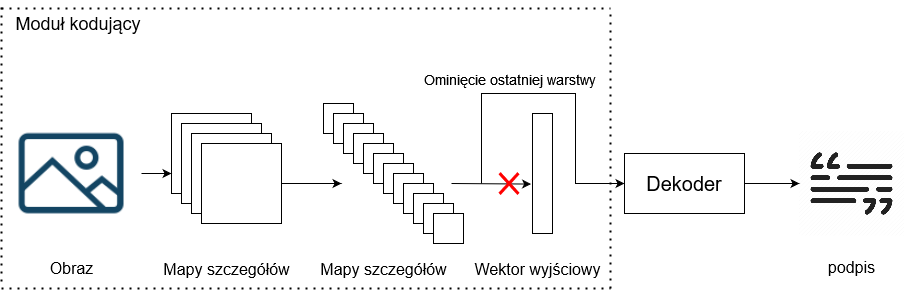
\includegraphics[width=\linewidth]{schemat-pretrained}
    \caption{Diagram przedstawiający architekturę z wykorzystanie wcześniej wyuczonych modeli jako modułów kodujących. Opracowanie własne.}
    \label{fig:schemat-pretrained}
\end{figure}
\noindent Wykorzystane moduły dekodujące:
\begin{itemize}
    \item RNN \cite{rnn} -- podstawowa rekurencyjna sieć neuronowa.
    \item LSTM \cite{lstm} -- jest rozszerzeniem podstawowej rekurencyjnej sieci neuronowej, której głównym celem jest rozwiązanie problemu zanikającego gradientu.
    \item GRU \cite{gru} -- posiada mniej parametrów niż LSTM, co w teorii pozwala na szybsze i wydajniejsze uczenie się.
    \item Transformer \cite{transformer} -- umożliwia na analizowanie pełnej sekwencji w jednym momencie poprzez wykorzystanie modułu atencji.
\end{itemize}
Każda kombinacja modułu kodującego wraz z modułem dekodującym została sprawdzona pod względem:
\begin{itemize}
    \item wydajności uczenia poprzez sprawdzenie czasu potrzebnego na przetworzenie przez architekturę treningowego zbioru danych,
    \item wydajności generowania podpisów, poprzez sprawdzenie czasu potrzebnego na przetworzenie testowego zbioru danych,
    \item efektywności poprzez sprawdzenie skuteczności generowania podpisów.
\end{itemize}
Wydajność testowania oraz skuteczność generowania podpisów została również sprawdzona dla dedykowanej architektury GIT \cite{wang2022git} wykorzystującej transformer wizyjny wraz z klasycznym transformerem. W tym celu wykorzystane zostały wagi udostępnione przez autorów -- pozwoliło to na całkowite pominięcie etapu uczenia tejże sieci.
\subsection{Trenowanie pełnej architektury}
W celu sprawdzenia jak duże znaczenie ma wykorzystanie wstępnie wytrenowanych modułów kodujących, ich wydajność treningowa została porównana do wydajności uczenia pełnej architektury. Porównane zostały wszystkie wcześniej wymienione kombinacje modułów kodujących wraz z modułami dekodującymi. Oprócz tego do zbioru modułów dekodujących dodany został również podstawowy wariant splotowej sieci neuronowej. Moduły zostały połączone w taki sam sposób jak w przypadku wykorzystania wstępnie wytrenowanych wag -- ostatnia warstwa w pełni połączona została usunięta, a dane wyjściowe modułu kodującego są bezpośrednimi danymi wejściowymi modułu dekodującego.
\subsection{Wstępne przetwarzanie danych}
Dane wejściowe w postaci macierzy pikseli obrazów cyfrowych zostały normalizowane, a ich wymiary ujednolicone w celu uproszczenia obliczeń. Natomiast przetwarzanie języka naturalnego odbyło się poprzez zastosowanie tokenizacji -- w tym celu został wykorzystany wcześniej wytrenowany model Distilbert \cite{distilbert}.
\subsection{Metryki}
Oprócz parametrów dotyczących wydajności trenowania oraz testowania podanych rozwiązań sprawdzona została również skuteczność otrzymanych wyników. Wybrane metryki:
\begin{itemize}
    \item BLEU (ang. Bilingual Evaluation Understudy) \cite{bleu} -- metryka oryginalnie wywodząca się z dziedziny tłumaczenia maszynowego, jednakże ze względu na taki sam format danych, idealnie pasuje również do ewaluacji wyników generowania podpisów do obrazów. Zakres wartości metryki zawiera się w przedziale od 0 do 1, gdzie najlepszą wartością jest górna granica. % MAYBE dodać formułe wyliczania oraz informację o n gramach
    \item METEOR (ang. Metric for Evaluation of Translation with Explicit ORdering) \cite{meteor} -- metryka będąca rozwinięciem metryki BLEU. Odznacza się lepszą oceną korelacji na poziomie zdań, a nie tak jak w~przypadku BLEU, na~poziomie całego korpusu. Zakres wartości metryki zawiera się w przedziale od 0 do 1, gdzie najlepszą wartością jest górna granica.
    \item CIDEr (ang. Consensus-based Image Description Evaluation) \cite{cider} -- dedykowana metryka do oceny jakości generowanych opisów obrazów. Poprzez zastosowanie algorytmu TF-IDF \cite{tfidf} pozwala na ocenę jakości generowanych podpisów w oparciu o~podobieństwo do wszystkich podpisów, a nie tylko do jednego. Zakres jej wartości jest większy niż w przypadku pozostałych metryk, ponieważ wynosi od 0 do 10, gdzie wartość 10 oznacza najlepszy wynik.
    \item SPICE -- wykorzystuje ona rozbiór logiczny zdania w celu stworzenie jego grafu, które są następnie porównywane z grafami pozostałych zdań. Dzięki temu metryka ta jest w stanie ocenić podobieństwo poprzez strukturę zdania, a nie tylko występowanie danych słów. Tak jak w przypadku metryk BLEU i METEOR zakres wartości zawiera się w przedziale od 0 do 1, gdzie najlepszą wartością jest górna granica.
\end{itemize}
W przypadku wyników architektur wykorzystujących różne kombinacje modułów kodujących oraz dekodujących zostały one przedstawione poprzez tylko dwie metryki: BLEU i CIDEr. Pozostałe wskaźniki zostały wykorzystane jedynie w przypadku porównania wyników bezpośrednio z wartościami otrzymanymi przez autorów dla dedykowanych rozwiązań. Ograniczenie zostało wprowadzone, w celu zachowania przejrzystości wyników, a także ze względu na fakt, iż metryki BLEU i CIDEr powinny być w pełni wystarczające, aby ocenić jakość generowanych podpisów.
\subsection{Wykorzystane środowiska}
W celu porównania wpływu użytych jednostek obliczeniowych na efektywność badanych architektury wykorzystane zostały różne karty graficzne:
\begin{itemize}
    \item NVIDIA GeForce GTX 1650 4GB -- jednostka GPU,
    \item NVIDIA Tesla T4 16 GB -- jednostka GPU,
    \item Intel Core i7-1280P -- jednostka CPU.
\end{itemize}
W przypadku karty graficznej Tesla T4 wszelkie testy zostały wykonane za pośrednictwem platformy Google Colab umożliwiającej bezpłatny dostęp do zaawansowanych jednostek obliczeniowych. Pozostałe testy zostały wykonane na komputerze osobistym

Docelowa architektura została zaimplementowana przy użyciu gotowych modeli sieci neuronowych zawartych w bibliotekach PyTorch \cite{pytorch} oraz Transformers \cite{wolf-etal-2020-transformers} dostępnych w języku programowania Python.
\subsection{Zbiory danych}
Istnieje wiele zbiorów danych zawierających obrazy wraz z ich opisami. Jednymi z najpopularniejszych są:
\begin{itemize}
    \item MS COCO \cite{mscoco} -- składa się on z ponad 120 tysięcy zdjęć.
    \item Flickr \cite{flickr30k} -- posiada on mniej zdjęć niż zbiór MS COCO, ponieważ jego szeroki wariant zawiera ich 30 tysięcy, natomiast węższy 8 tysięcy.
\end{itemize}
Ze względu na konieczność wytrenowania dużej liczby architektur niezwykle istotne jest dokonanie tego w sensownym oknie czasowym, co może być niewykonalne przy wykorzystaniu zbioru MS COCO. Z tego względu został wykorzystany węższy wariant zbioru Flickr zawierający 8 tysięcy zdjęć. Ten wybór pozwolił również sprawdzić skuteczność modelu GIT bez wcześniejszego go wytrenowania, posługując się jedynie modelem udostępnionym przez autorów, który został wytrenowany na zbiorze MS COCO.
Zbiór danych został podzielony na:
\begin{itemize}
    \item zbiór treningowy -- 6 tysięcy zdjęć,
    \item zbiór testowy -- 1 tysiąc zdjęć,
    \item zbiór walidacyjny -- 1 tysiąc zdjęć.
\end{itemize}

\noindent Wszystkie kombinacje wykorzystanych architektur zostały wyuczone przy pomocy treningowego zbioru danych. Dodatkowo w trakcie treningu jakość modelu była sprawdzana przy pomocy zbioru walidacyjnego. Dane były przetwarzane w seriach liczących po 32 elementy. Przetwarzanie było powtarzane 500 razy.
